% 图 6.1 —— 由 `checks/emit_hand.py` 自动拼出（probe 精测 + prims2 图元分解）
%%
% ⚠ 这是**稿子不是成品**：跑 `checks/checkhand.py 6.1` 看指标 + 看叠合图。
%%
%% ★★ 2026-09-18 已**人工定稿** —— 重跑 `emit_hand.py --force 6.1` 会**丢掉下面这些**：
%%    · 四个箭头的实心三角头（prims2 没把箭头三角识别成 fill，只给了两根倒刺 + 一坨糊块）
%%      → 改用 TikZ 标准 Tip：`-{Triangle[width=14pt,length=21pt]}`，并删掉原来的 18 行残笔
%%    · 上面「去掉 (190.0,131.0)--(190.0,189.0) 等 18 行」的手工删除
%%    要重跑出稿的话，**跑完必须把这份草稿的改动重新贴回去**。
%%    （标签部分的修正已落进 `texts_6.1.json`（manual:true），重跑不会丢。）
%%
%% ⚠ 待核：
%   · 本图 probe 报出阴影族 1 个 —— **本脚本不生成阴影**（要照原书手写）；prims2 的 strokes 里可能含阴影线，核对时留意别画重
%   · 可疑字形 1 项（空心圈 ⊙ 常被认成字母 o）—— 见文件末
%%
\documentclass[12pt]{standalone}
\usepackage{fontspec}
\setsansfont{Arial}
\newfontfamily\mfallback{DejaVu Sans}
\usepackage{tikz}
\usetikzlibrary{arrows.meta}
\begin{document}
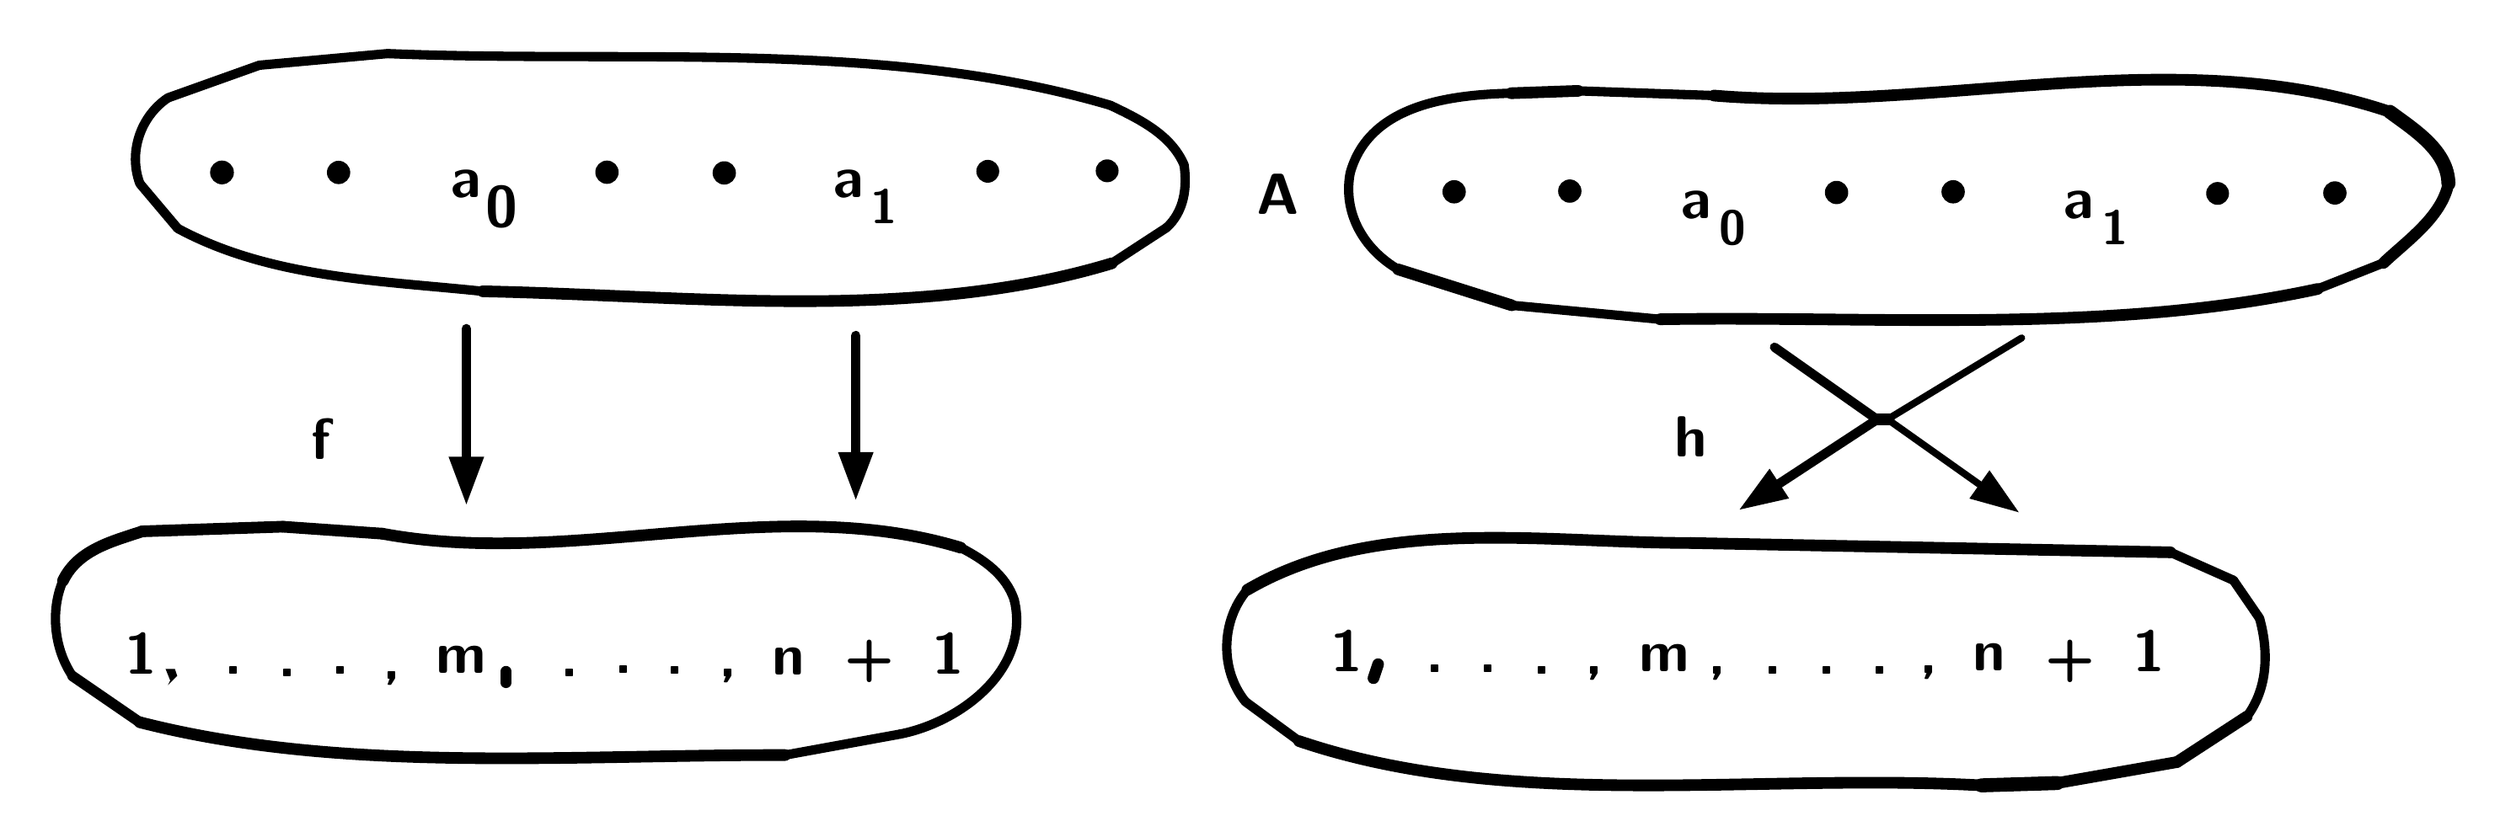
\begin{tikzpicture}[x=1pt, y=-1pt, line width=3.0pt, line cap=round, line join=round]

  %% ════ 填充区（prims2 的 fills）════
  \fill (65.0,277.0) -- (61.0,277.0) -- (63.0,282.0) -- (62.0,284.0) -- (66.0,280.0) -- cycle;

  %% ════ 直线段（prims2 的 strokes）════
  \draw[line width=3.0pt] (801.0,169.0) -- (857.0,135.0);
  \draw[line width=5.0pt] (800.0,170.0) -- (795.0,170.0);
  \draw[line width=4.0pt] (795.0,170.0) -- (751.0,139.0);
  \draw[line width=5.0pt] (581.0,275.0) -- (579.0,281.0);
  \draw[line width=4.5pt] (207.0,278.0) -- (207.0,283.0);
  \draw[line width=4.0pt] (376.0,305.0) -- (326.7,314.0);
  \draw[line width=4.5pt] (49.9,299.9) -- (21.1,280.1);
  \draw[line width=5.0pt] (51.0,218.0) -- (111.2,216.0);
  \draw[line width=5.0pt] (111.2,216.0) -- (154.0,219.0);
  \draw[line width=4.0pt] (524.1,291.1) -- (547.1,308.0);
  \draw[line width=6.0pt] (839.7,327.0) -- (872.3,326.0);
  \draw[line width=5.0pt] (872.3,326.0) -- (923.6,317.0);
  \draw[line width=5.0pt] (923.6,317.0) -- (953.5,297.5);
  \draw[line width=4.0pt] (959.0,255.3) -- (947.8,239.0);
  \draw[line width=4.0pt] (947.8,239.0) -- (920.8,227.0);
  \draw[line width=5.0pt] (920.8,227.0) -- (715.0,223.0);
  \draw[line width=5.0pt] (589.6,105.6) -- (638.3,121.0);
  \draw[line width=4.0pt] (638.3,121.0) -- (701.9,127.0);
  \draw[line width=4.0pt] (983.9,114.0) -- (1012.2,102.8);
  \draw[line width=4.0pt] (725.0,31.0) -- (666.8,29.0);
  \draw[line width=5.0pt] (666.8,29.0) -- (638.0,30.0);
  \draw[line width=4.0pt] (66.2,88.0) -- (50.0,68.8);
  \draw[line width=4.0pt] (62.0,32.0) -- (101.2,18.0);
  \draw[line width=4.0pt] (101.2,18.0) -- (156.2,13.0);
  \draw[line width=4.0pt] (490.4,87.6) -- (466.8,103.0);

  %% ── 2026-09-18 手工定稿：四个箭头的实心三角头 ──
  %% 原稿把头描成了两根倒刺 + 一坨糊块（prims2 没把实心三角识别成 fill），
  %% 这里改用 TikZ 标准箭头 Tip（arrows.meta 的 Triangle），尺寸按原书墨迹剖面量的：
  %%   头宽 14pt、头长 21pt。
  \draw[line width=4.0pt,-{Triangle[width=14pt,length=21pt]}] (190.0,131.0) -- (190.0,207.0);
  \draw[line width=4.0pt,-{Triangle[width=14pt,length=21pt]}] (357.0,134.0) -- (357.0,205.0);
  \draw[line width=4.0pt,-{Triangle[width=14pt,length=21pt]}] (795.0,170.0) -- (735.5,209.0);
  \draw[line width=3.0pt,-{Triangle[width=14pt,length=21pt]}] (801.0,171.0) -- (856.0,210.0);

  %% ════ 曲线（prims2 的 curves —— 三段式，坐标同为 (y,x)）════
  \draw[line width=5.0pt] (326.7,314.0) .. controls (233.6,313.8) and (136.8,322.2) .. (49.9,299.9);
  \draw[line width=4.0pt] (21.1,280.1) .. controls (13.2,268.5) and (11.5,252.1) .. (17.0,239.2);
  \draw[line width=5.0pt] (17.0,239.2) .. controls (23.4,225.8) and (38.5,222.2) .. (51.0,218.0);
  \draw[line width=5.0pt] (154.0,219.0) .. controls (235.6,234.2) and (322.5,200.8) .. (402.0,225.0);
  \draw[line width=4.0pt] (402.0,225.0) .. controls (411.7,230.0) and (421.5,236.7) .. (425.0,247.6);
  \draw[line width=4.0pt] (425.0,247.6) .. controls (431.9,277.5) and (401.8,299.9) .. (376.0,305.0);
  \draw[line width=5.0pt] (715.0,223.0) .. controls (651.3,222.9) and (579.7,211.0) .. (524.9,243.1);
  \draw[line width=4.0pt] (524.9,243.1) .. controls (513.5,256.4) and (513.1,277.5) .. (524.1,291.1);
  \draw[line width=5.0pt] (547.1,308.0) .. controls (637.6,338.7) and (742.5,321.6) .. (839.7,327.0);
  \draw[line width=4.0pt] (953.5,297.5) .. controls (962.7,285.3) and (962.9,269.3) .. (959.0,255.3);
  \draw[line width=4.0pt] (638.0,30.0) .. controls (611.6,30.7) and (577.1,34.9) .. (569.0,64.3);
  \draw[line width=4.0pt] (569.0,64.3) .. controls (565.8,81.7) and (575.0,97.0) .. (589.6,105.6);
  \draw[line width=5.0pt] (701.9,127.0) .. controls (796.3,125.5) and (894.3,133.4) .. (983.9,114.0);
  \draw[line width=5.0pt] (1012.2,102.8) .. controls (1022.7,92.9) and (1037.0,83.1) .. (1040.0,68.8);
  \draw[line width=6.0pt] (1040.0,68.8) .. controls (1039.7,54.5) and (1025.1,45.6) .. (1014.9,38.0);
  \draw[line width=5.0pt] (1014.9,38.0) .. controls (923.1,7.0) and (820.6,39.0) .. (725.0,31.0);
  \draw[line width=4.0pt] (197.0,115.0) .. controls (152.1,110.3) and (105.6,109.3) .. (66.2,88.0);
  \draw[line width=4.0pt] (50.0,68.8) .. controls (45.0,55.6) and (50.1,40.0) .. (62.0,32.0);
  \draw[line width=4.0pt] (156.2,13.0) .. controls (260.9,17.3) and (369.7,6.7) .. (466.2,35.2);
  \draw[line width=4.0pt] (466.2,35.2) .. controls (478.1,40.9) and (492.2,47.6) .. (497.8,60.8);
  \draw[line width=4.0pt] (497.8,60.8) .. controls (499.2,70.9) and (497.7,80.7) .. (490.4,87.6);
  \draw[line width=5.0pt] (466.8,103.0) .. controls (382.7,128.5) and (286.6,116.8) .. (197.0,115.0);

  %% ════ 实心点 ════
  \fill (85.2,64.0) circle (5.1);
  \fill (135.2,64.0) circle (5.0);
  \fill (250.3,63.9) circle (5.0);
  \fill (300.6,64.2) circle (5.0);
  \fill (413.6,63.5) circle (4.9);
  \fill (464.8,63.3) circle (4.9);
  \fill (613.6,72.3) circle (5.0);
  \fill (663.2,72.0) circle (5.0);
  \fill (777.6,72.6) circle (5.0);
  \fill (827.6,72.3) circle (5.0);
  \fill (941.0,73.0) circle (4.9);
  \fill (991.3,72.8) circle (5.0);

  %% ════ 标签（probe 直接给的 \node 行）════
  %% ⚠ 全部补了 fill=white：文字在最上层，否则与曲线交叉干扰
     \node[anchor=center,inner sep=0pt,fill=white,font=\fontsize{29.9}{37.4}\selectfont] at (190.0,69.0) {\textsf{\textbf{\textit{a}}}};   % box(182,59,14,17)
     \node[anchor=center,inner sep=0pt,fill=white,font=\fontsize{29.9}{37.4}\selectfont] at (354.0,69.0) {\textsf{\textbf{\textit{a}}}};   % box(346,59,14,17)
     \node[anchor=center,inner sep=0pt,fill=white,font=\fontsize{29.6}{37.0}\selectfont] at (538.2,73.5) {\textsf{\textbf{\textit{A}}}};   % box(526,62,19,22)
     \node[anchor=center,inner sep=0pt,fill=white,font=\fontsize{28.8}{36.0}\selectfont] at (717.5,77.9) {\textsf{\textbf{\textit{a}}}};   % box(710,68,13,17)
     \node[anchor=center,inner sep=0pt,fill=white,font=\fontsize{28.8}{36.0}\selectfont] at (881.5,77.9) {\textsf{\textbf{\textit{a}}}};   % box(874,68,13,17)
     \node[anchor=center,inner sep=0pt,fill=white,font=\fontsize{24.9}{31.1}\selectfont] at (205.1,78.7) {\textsf{\textbf{0}}};   % box(197,70,12,17)
     \node[anchor=center,inner sep=0pt,fill=white,font=\fontsize{21.5}{26.9}\selectfont] at (369.0,78.9) {\textsf{\textbf{1}}};   % box(363,71,7,15)
     \node[anchor=center,inner sep=0pt,fill=white,font=\fontsize{22.7}{28.4}\selectfont] at (732.9,87.7) {\textsf{\textbf{0}}};   % box(726,79,10,17)
     \node[anchor=center,inner sep=0pt,fill=white,font=\fontsize{21.5}{26.9}\selectfont] at (897.0,87.9) {\textsf{\textbf{1}}};   % box(891,80,7,15)
     \node[anchor=center,inner sep=0pt,fill=white,font=\fontsize{30.3}{37.9}\selectfont] at (715.3,177.5) {\textsf{\textbf{\textit{h}}}};   % box(707,165,16,22)
     \node[anchor=center,inner sep=0pt,fill=white,font=\fontsize{27.1}{33.9}\selectfont] at (128.5,178.5) {\textsf{\textbf{\textit{f}}}};   % box(123,167,10,22)
     \node[anchor=center,inner sep=0pt,fill=white,font=\fontsize{29.7}{37.1}\selectfont] at (567.5,269.5) {\textsf{\textbf{1}}};   % box(559,259,10,20)
     \node[anchor=center,inner sep=0pt,fill=white,font=\fontsize{29.7}{37.1}\selectfont] at (911.5,269.5) {\textsf{\textbf{1}}};   % box(903,259,10,20)
     \node[anchor=center,inner sep=0pt,fill=white,font=\fontsize{29.7}{37.1}\selectfont] at (50.5,270.5) {\textsf{\textbf{1}}};   % box(42,260,10,20)
     \node[anchor=center,inner sep=0pt,fill=white,font=\fontsize{29.7}{37.1}\selectfont] at (396.5,270.5) {\textsf{\textbf{1}}};   % box(388,260,10,20)
     \node[anchor=center,inner sep=0pt,fill=white,font=\fontsize{30.3}{37.9}\selectfont] at (703.8,272.3) {\textsf{\textbf{\textit{m}}}};   % box(691,262,24,17)
     \node[anchor=center,inner sep=0pt,fill=white,font=\fontsize{29.9}{37.4}\selectfont] at (843.2,272.2) {\textsf{\textbf{\textit{n}}}};   % box(835,262,15,17)
     \node[anchor=center,inner sep=0pt,fill=white,font=\fontsize{30.3}{37.9}\selectfont] at (187.8,273.3) {\textsf{\textbf{\textit{m}}}};   % box(175,263,24,17)
     \node[anchor=center,inner sep=0pt,fill=white,font=\fontsize{30.8}{38.5}\selectfont] at (328.3,273.8) {\textsf{\textbf{\textit{n}}}};   % box(320,263,15,18)
     \node[anchor=center,inner sep=0pt,fill=white,font=\fontsize{32.0}{40.0}\selectfont] at (362.9,273.9) {\textsf{\textbf{+}}};   % box(353,264,16,16)
     \node[anchor=center,inner sep=0pt,fill=white,font=\fontsize{32.0}{40.0}\selectfont] at (877.9,273.9) {\textsf{\textbf{+}}};   % box(868,264,16,16)
     \node[anchor=center,inner sep=0pt,fill=white,font=\fontsize{39.9}{49.8}\selectfont] at (817.3,278.7) {\textsf{\textbf{,}}};   % box(812,273,6,10)
     \node[anchor=center,inner sep=0pt,fill=white,font=\fontsize{45.0}{56.2}\selectfont] at (257.4,277.4) {\textsf{\textbf{.}}};   % box(251,274,6,6)
     \node[anchor=center,inner sep=0pt,fill=white,font=\fontsize{37.5}{46.9}\selectfont] at (605.3,276.8) {\textsf{\textbf{.}}};   % box(600,274,5,5)
     \node[anchor=center,inner sep=0pt,fill=white,font=\fontsize{37.5}{46.9}\selectfont] at (628.3,276.8) {\textsf{\textbf{.}}};   % box(623,274,5,5)
     \node[anchor=center,inner sep=0pt,fill=white,font=\fontsize{34.5}{43.1}\selectfont] at (673.5,279.1) {\textsf{\textbf{,}}};   % box(669,274,5,9)
     \node[anchor=center,inner sep=0pt,fill=white,font=\fontsize{34.5}{43.1}\selectfont] at (726.5,279.1) {\textsf{\textbf{,}}};   % box(722,274,5,9)
     \node[anchor=center,inner sep=0pt,fill=white,font=\fontsize{41.1}{51.3}\selectfont] at (90.1,277.8) {\textsf{\textbf{.}}};   % box(84,275,6,5)
     \node[anchor=center,inner sep=0pt,fill=white,font=\fontsize{41.1}{51.3}\selectfont] at (136.1,277.8) {\textsf{\textbf{.}}};   % box(130,275,6,5)
     \node[anchor=center,inner sep=0pt,fill=white,font=\fontsize{37.5}{46.9}\selectfont] at (279.3,277.8) {\textsf{\textbf{.}}};   % box(274,275,5,5)
     \node[anchor=center,inner sep=0pt,fill=white,font=\fontsize{37.8}{47.3}\selectfont] at (302.2,280.1) {\textsf{\textbf{,}}};   % box(297,275,6,9)
     \node[anchor=center,inner sep=0pt,fill=white,font=\fontsize{37.5}{46.9}\selectfont] at (651.3,277.8) {\textsf{\textbf{.}}};   % box(646,275,5,5)
     \node[anchor=center,inner sep=0pt,fill=white,font=\fontsize{37.5}{46.9}\selectfont] at (750.3,277.8) {\textsf{\textbf{.}}};   % box(745,275,5,5)
     \node[anchor=center,inner sep=0pt,fill=white,font=\fontsize{37.5}{46.9}\selectfont] at (773.3,277.8) {\textsf{\textbf{.}}};   % box(768,275,5,5)
     \node[anchor=center,inner sep=0pt,fill=white,font=\fontsize{37.5}{46.9}\selectfont] at (796.3,277.8) {\textsf{\textbf{.}}};   % box(791,275,5,5)
     \node[anchor=center,inner sep=0pt,fill=white,font=\fontsize{37.5}{46.9}\selectfont] at (113.3,278.8) {\textsf{\textbf{.}}};   % box(108,276,5,5)
     \node[anchor=center,inner sep=0pt,fill=white,font=\fontsize{37.8}{47.3}\selectfont] at (158.2,281.1) {\textsf{\textbf{,}}};   % box(153,276,6,9)
     \node[anchor=center,inner sep=0pt,fill=white,font=\fontsize{37.5}{46.9}\selectfont] at (234.3,278.8) {\textsf{\textbf{.}}};   % box(229,276,5,5)

  % 钉死画布：否则超出的图元/控制点会把页面撑大，1:1 回比就失准
  \pgfresetboundingbox
  \path[use as bounding box] (0,0) rectangle (1052,337);
\end{tikzpicture}
\end{document}

% ⚠ 待核清单（probe 拿不准，人眼过一遍）：
%   · 未识别/跳过：⑤ 跳过/未识别的字形
